\section{\textit{Event-Driven Architecture}}

\textit{Event-driven architecture} merupakan paradigma arsitektur perangkat lunak yang berkaitan dengan produksi dan deteksi \textit{events}. Arsitektur ini mudah dievolusikan dan menawarkan \textit{fault tolerance}, kinerja yang baik, dan \textit{scalability}. Meskipun begitu, arsitektur ini kompleks dan sulit untuk diuji. Arsitektur ini cocok untuk kasus yang kompleks dan dinamis \parencite{softwareArchitecture}.

Arsitektur ini terdiri atas tiga komponen, yaitu \textit{event producer}, \textit{event router}, dan \textit{event consumer}. Sebuah \textit{producer} mengirimkan \textit{event} ke \textit{router}, lalu di-\textit{filter} dan dikirimkan kepada \textit{consumer}.

\subsection{Redpanda}

Redpanda merupakan \textit{event streaming platform}. Platform ini menyediakan infrastruktur untuk \textit{streaming real-time data}. Produsen mengirimkan data berupa \textit{event} ke Redpanda, kemudian Redpanda menyimpan \textit{event} tersebut lalu mengaturnya ke dalam sebuah topik. Topik ini merupakan log \textit{event} yang dapat diputar ulang. Konsumen mengonsumsi \textit{event} pada topik Redpanda secara asinkron \parencite{redpandaIntro}.

\begin{figure}[htbp]
    \centering
    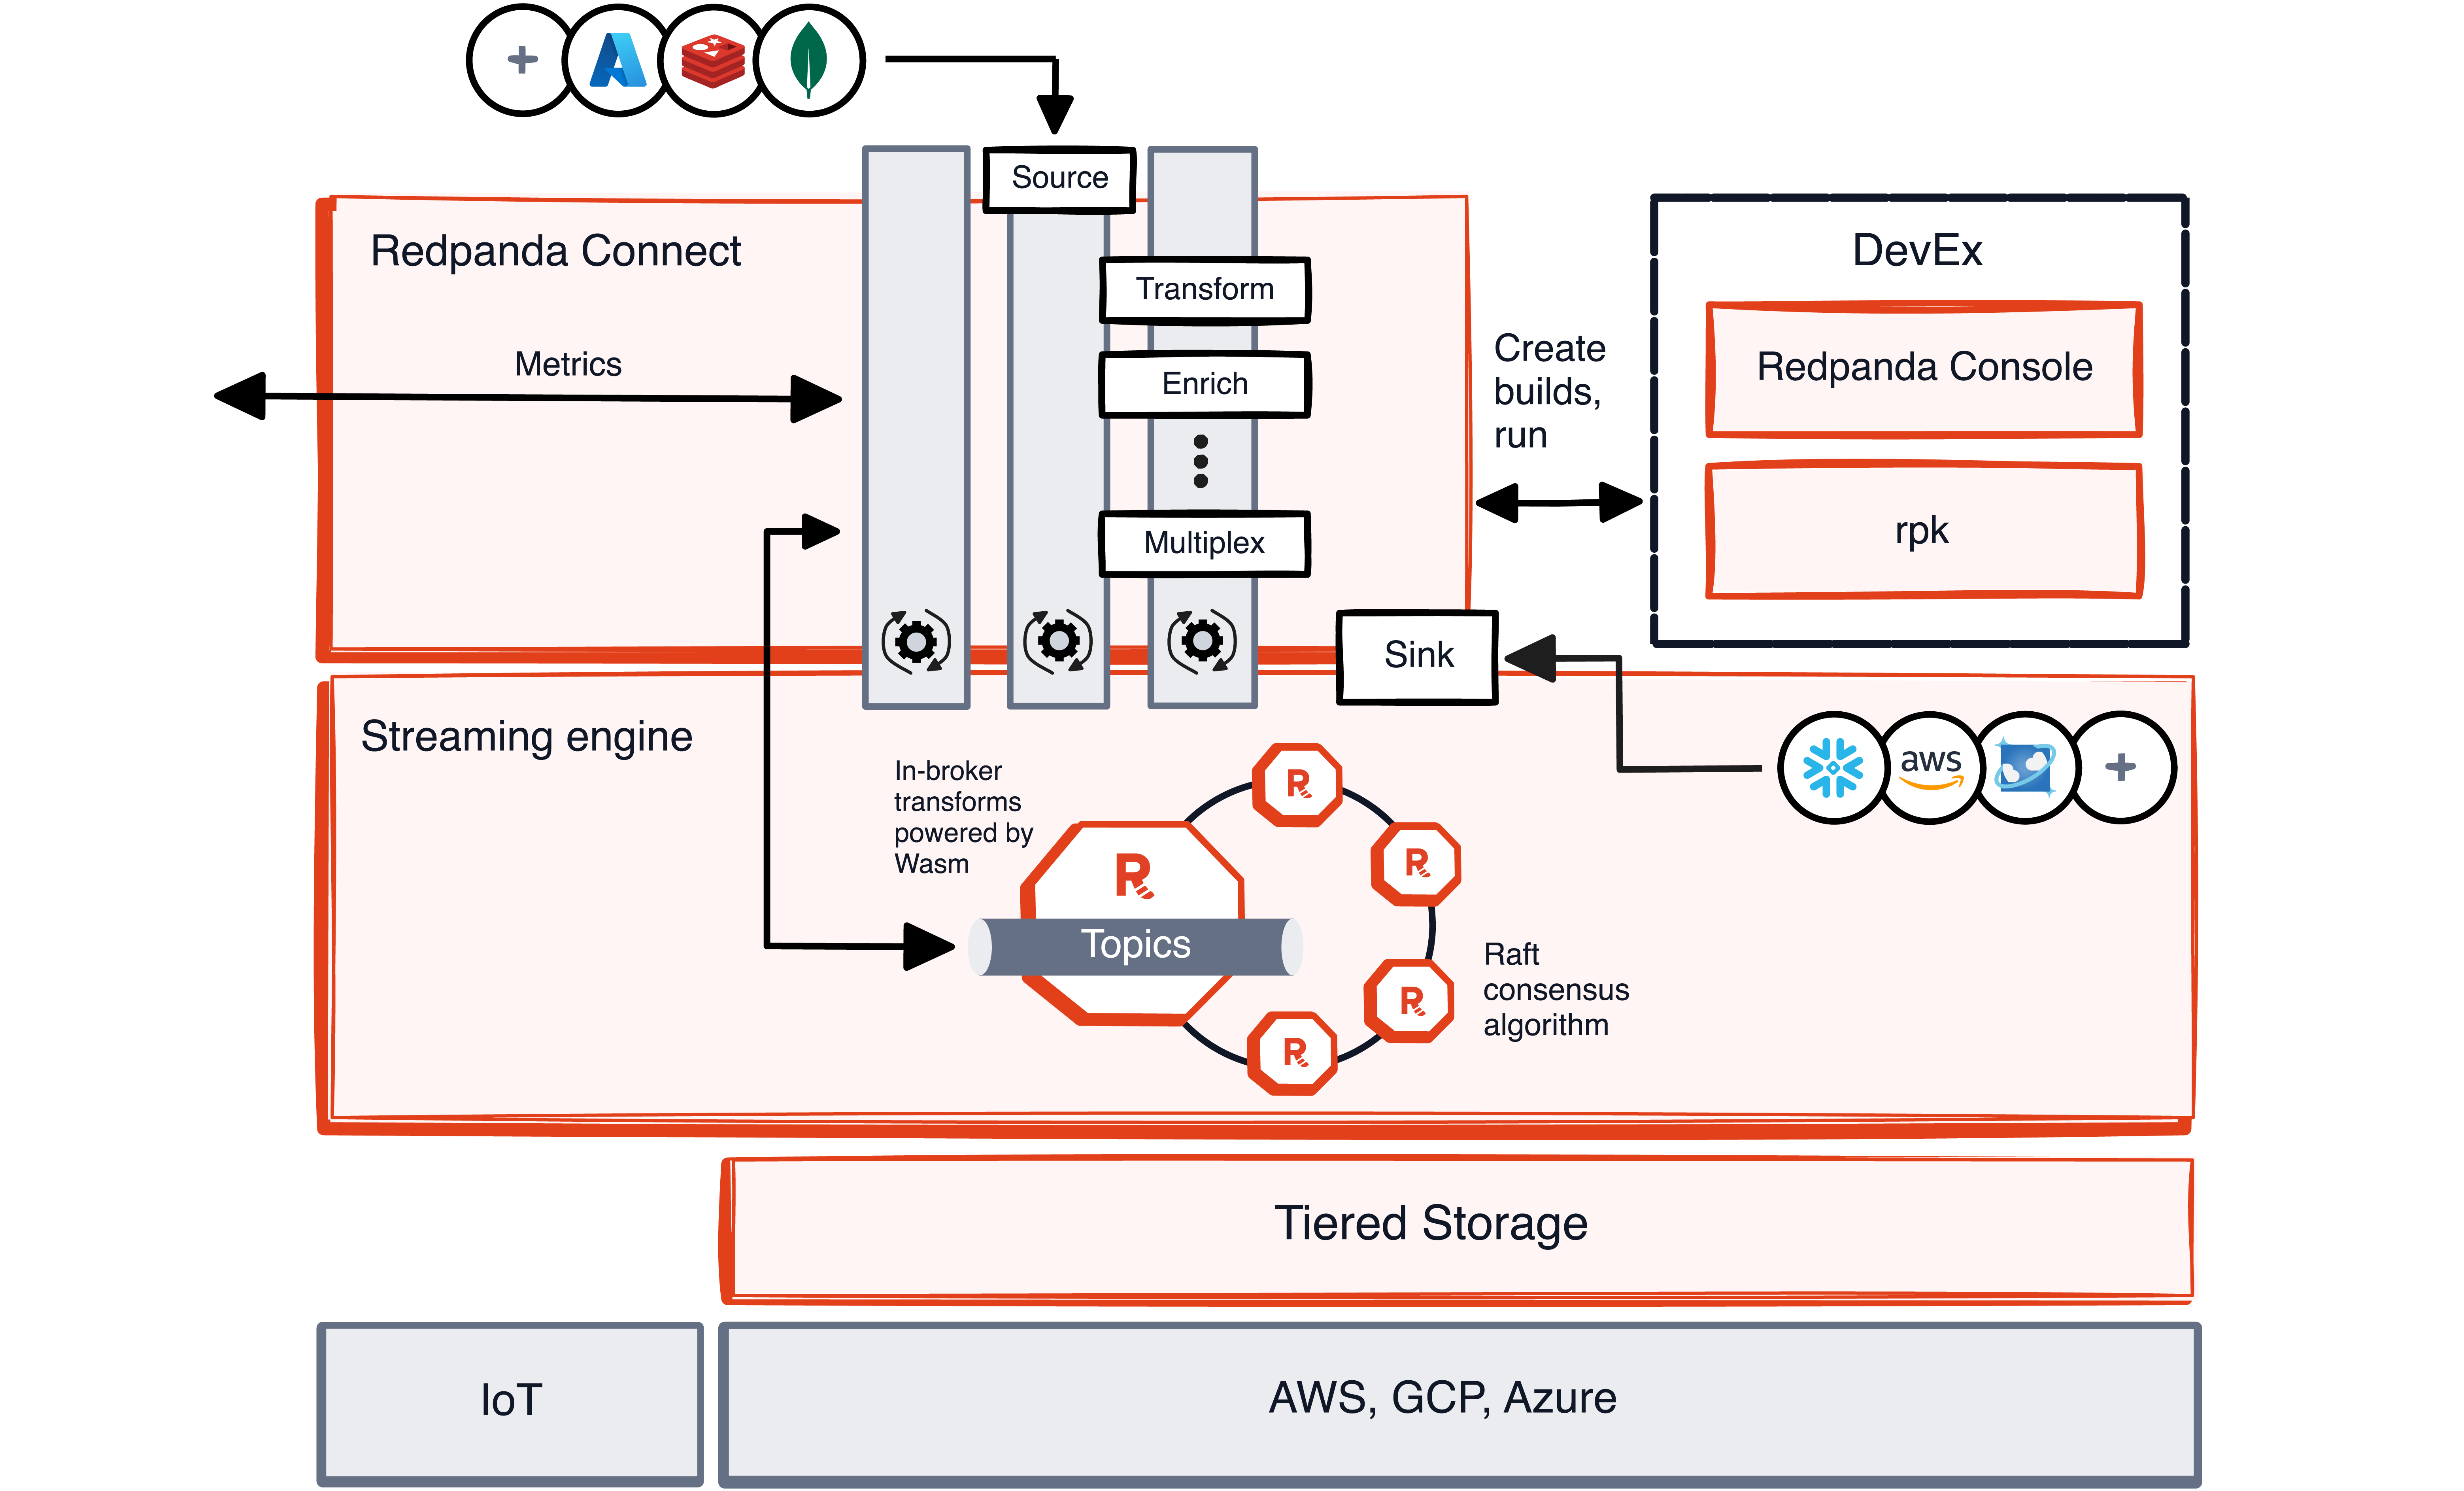
\includegraphics[width=0.8\textwidth]{resources/chapter-2/redpanda.png}
    \caption{Apa itu Redpanda? \parencite{whatIsRedpanda}}
    \label{fig:what-is-redpanda}
\end{figure}

Redpanda merupakan \textit{event streaming platform} alternatif dari Apache Kafka. Selain itu, platform ini menawarkan kompatibilitas API yang sama dengan Kafka sehingga memudahkan migrasi penggunanya. Meskipun begitu, terdapat beberapa perbedaan antara Redpanda dengan Apache Kafka.

Perbedaan pertama adalah algoritma konsensus yang digunakan. Apache Kafka menggunakan ZooKeeper (versi lama) sedangkan Redpanda menggunakan Raft. Meskipun begitu, versi terbaru Kafka sudah menggunakan algoritma konsensus Kraft yang merupakan varian dari Raft dengan perbedaan pada mekanisme replikasi log \parencite{raftKraft}.

Selain itu, Redpanda berfokus pada pengoptimalan kinerja yang lebih baik dibandingkan dengan Apache Kafka. Redpanda ditulis dalam bahasa C++, sedangkan Apache Kafka ditulis dalam bahasa Java dan berjalan pada JVM. Dalam hal ini, Redpanda menggunakan bahasa sistem sehingga minim \textit{overhead}.

Berikut adalah contoh pengoptimalan yang dilakukan pada Redpanda: \textit{Direct Memory Access (DMA)} untuk I/O, distribusi pemrosesan \textit{interrupt request} (IRQ) pada beberapa core CPU, penggunaan model \textit{thread per core}, dan pengoptimalan lainnya. Penggunaan model \textit{thread per core} memungkinkan Redpanda untuk menjalankan \textit{thread} aplikasi pada inti CPU yang sama sehingga \textit{context switching} dan \textit{blocking} dapat dihindari \parencite{redpandaArchitecture}.

\subsection{\textit{Change Data Capture}}

Menurut \cite{dataIntensiveApplications}, \textit{change data capture (CDC)} merupakan sebuah proses yang mengobservasi setiap perubahan pada data yang ditulis ke dalam basis data dan mengekstraknya ke dalam bentuk yang bisa direplikasi oleh sistem lain. Sebagai contoh, perubahan pada database bisa di-\textit{capture} lalu diterapkan pada \textit{search index} untuk menyamakan data pada basis data. Apabila \textit{log} diaplikasikan dalam urutan yang sama, data pada \textit{search index} dan basis data bisa dipastikan sama.

\begin{figure}[ht]
    \centering
    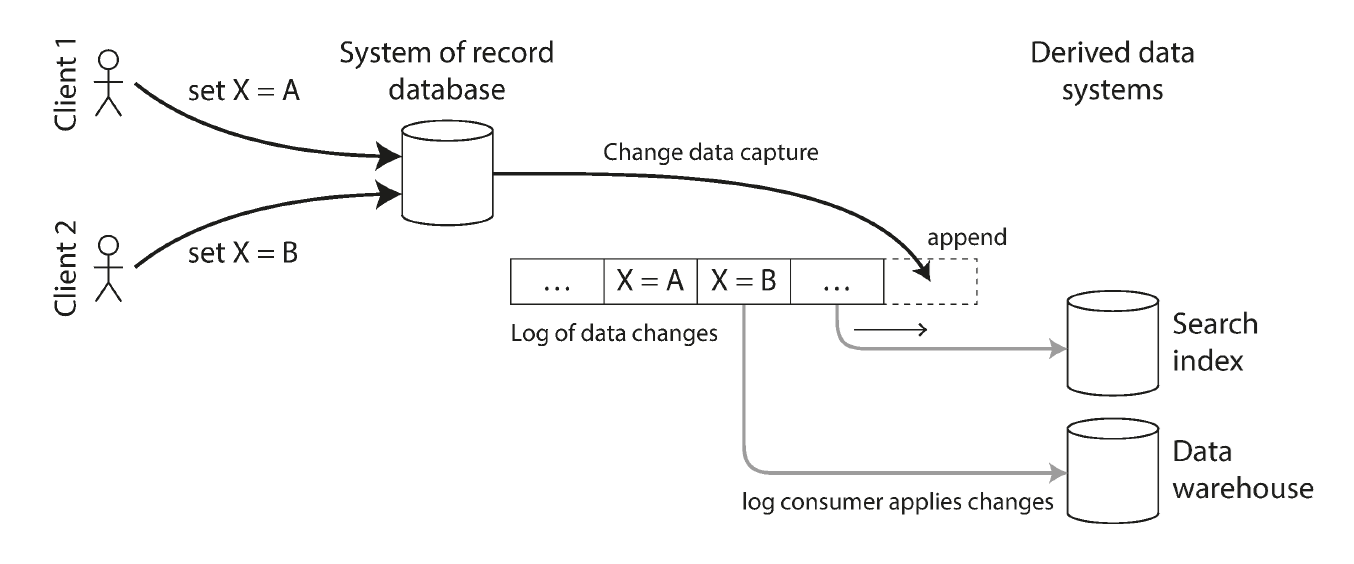
\includegraphics[width=0.8\textwidth]{resources/chapter-2/cdc.png}
    \caption{\textit{CDC Illustration \parencite{dataIntensiveApplications}}}
    \label{fig:cdc-illustration}
\end{figure}

PostgreSQL juga mendukung CDC dengan istilah \textit{logical replication}. Mekanisme ini menggunakan model \textit{publish} dan \textit{subscribe}. PostgreSQL yang mengirimkan \textit{log} bertindak sebagai \textit{publisher}, lalu terdapat \textit{subscriber} lain yang mengonsumsi \textit{log} yang dipublikasikan. \textit{Subscriber} ini bisa berupa replika PostgreSQL lagi atau aplikasi lainnya \parencite{pgLogicalReplication}. PostgreSQL mendukung dua mode operasi untuk replikasi, yaitu replikasi secara \textit{asynchronous} dan \textit{synchronous} \parencite{insideLogicalReplication}. Pada mode \textit{synchronous}, \textit{subscriber} harus merespons terlebih dahulu terhadap perubahan data sebelum PostgreSQL dapat melakukan \textit{commit}.

\begin{figure}[ht]
    \centering
    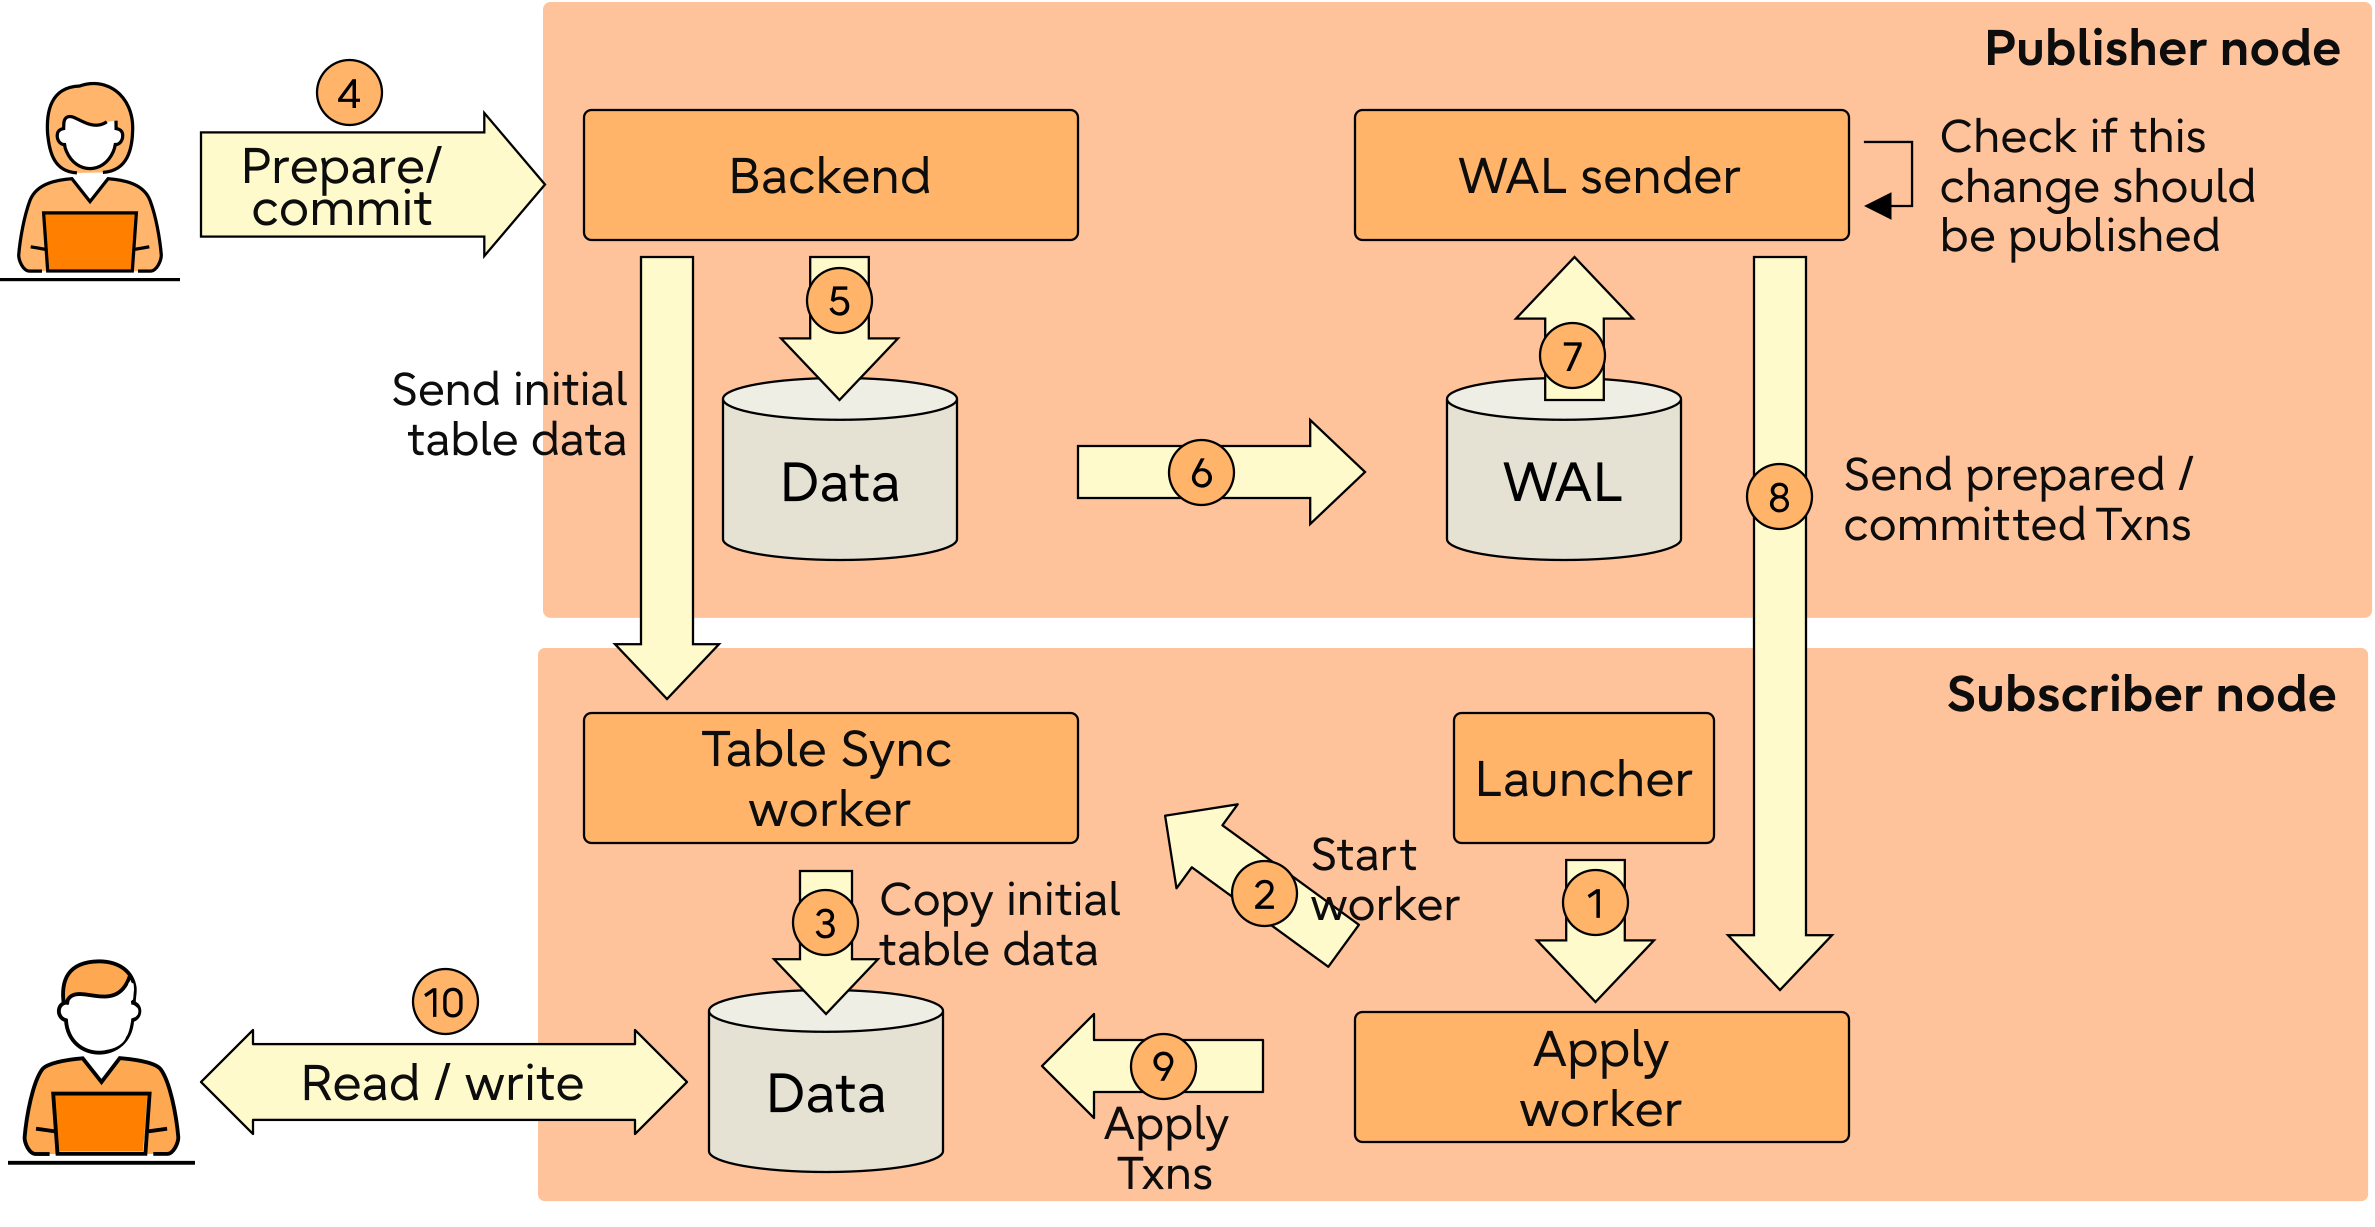
\includegraphics[width=0.8\textwidth]{resources/chapter-2/postgres-logical-replication.png}
    \caption{\textit{Logical Replication Architecture \parencite{insideLogicalReplication}}}
    \label{fig:logical-replication-architecture}
\end{figure}



\subsection{\textit{Event Sourcing}}

Mirip seperti \textit{change data capture}, \textit{event sourcing} juga menyimpan setiap perubahan pada \textit{state} aplikasi sebagai \textit{log of events}. Perbedaan terbesarnya terletak pada level abstraksinya. Pada \textit{change data capture}, aplikasi menggunakan basis data \textit{in a mutable way} dan dapat memperbarui atau menghapus \textit{record} sesuka hati. Aplikasi yang menulis pada basis data tidak harus \textit{aware} bahwa terdapat CDC. Berbeda dengan \textit{event sourcing}, logika aplikasi dibandung secara eksplisit di atas asumsi \textit{immutable event} yang ditulis pada \textit{event log}. Pada kasus ini, \textit{event} berupa \textit{append only}. Singkatnya, \textit{event sourcing} didesain untuk bisa merefleksikan hal yang terjadi pada level aplikasi dan bukan pada \textit{low-level state changes}.